\documentclass[11pt]{article}
\usepackage{epsfig}    % to insert postscript figures
\begin{document}

\title{Estimating $\mathcal{R}(t)$ from Covid-19 case counts}
\author{ Hugh Murrell}
\maketitle

\begin{abstract}
Here we attempt to give an interpretation of
the {\it effective reproduction number}, $\mathcal{R}_t$ that arises
from the Susceptible-Infected-Recovered (SIR) model 
for the spread of infectious disease.We also investigate how
 $\mathcal{R}_t$ may be estimated from daily case count data.
\end{abstract}

\section{Introduction}
The Susceptible-Infected-Recovered (SIR) model \cite{Wikipedia} is often used 
to study the spread of infectious disease by tracking the number (S) of people 
susceptible to the disease, the number (I) of people infected with the disease, 
and the number (R) of people who have had the disease and are now no
longer infectious.  

Based on the model, the only way that a person can leave the susceptible
group is to become infected, and the only way that a person can leave the
infected group is to recover or die.  It is further assumed that those
who have recovered or died from the disease are no longer susceptible.
 It is also assumed 
that all those who have not had the disease are equally susceptible
and that the probability of their contracting the disease at time $t$
is proportional to the product of $I(t)$ and $S(t)$. 

These assumptions lead us to a set of three ordinary differential equations
for $S(t)$, $I(t)$, and $R(t)$:

\begin{eqnarray}
\frac{dS}{dt} & = & - \gamma \mathcal{R}_t I(t) \label{eq2a} \\
\frac{dI}{dt} & = & \gamma \mathcal{R}_t I(t) - \gamma I(t) \label{eq2b} \\
\frac{dR}{dt} & = & \gamma I(t) . \label{eq2c}
\end{eqnarray}

Here $\gamma \geq 0$ is called the {\bf recovery rate}.
It is the reciprocal of the length of the infectious period which in the case of
Covid-19 is estimated to be about one week, so $\gamma = \frac{1}{7}$.

$\gamma \mathcal{R}_t \geq 0$ measures the likelihood
of transmitting the disease when an infected and a susceptible come
in contact.   Hence $\mathcal{R}_t$ is the number of transmissions
caused by an infected person during his infectious period.

section{Behavior of Groups over Time}
From equations (\ref{eq2a}-\ref{eq2c}) one can analyze equilibria -- where $dS/dt = 
dI/dt = dR/dt = 0$ -- using techniques in \cite[Sec. 9.2]{Tung}.  Equilibria 
occur when $I = 0$.  To see if they are stable we will linearize the
equations about $( I_{*} , S_{*} ) = (0, S_{*} )$.  [Note that equation (\ref{eq2c})
is really equivalent to $R(t) = N - I(t) - S(t)$.  Since $R$ is not involved
in the other two equations (\ref{eq2a}-\ref{eq2b}), we can ignore it for this analysis.]
Writing $S(t) = S_{*} + u(t)$ and $I(t) = I_{*} + v(t) = v(t)$, we see that $u$ and $v$
satisfy $dS/dt = du/dt = f(u,v)$ and $dI/dt = dv/dt = g(u,v)$,
where $f(u,v) = - \beta ( S_{*} + u ) v$ and 
$g(u,v) = [ \beta ( S_{*} + u ) - k] v$.  Expanding $f$ and $g$ in Taylor
series about $(0,0)$ and dropping terms involving $u^2$, $uv$, $v^2$, etc.,
we can write
\begin{eqnarray*}
f(u,v) & \approx & f(0,0) + \frac{\partial f}{\partial u} (0,0) \cdot u +
\frac{\partial f}{\partial v} (0,0) \cdot v = - \beta S_{*} v \\
g(u,v) & \approx & g(0,0) + \frac{\partial g}{\partial u} (0,0) \cdot u +
\frac{\partial g}{\partial v} (0,0) \cdot v = ( \beta S_{*} - k ) v .
\end{eqnarray*}
This leads to the linearized equations for $u$ and $v$:
\begin{eqnarray}
\frac{du}{dt} & = & - \beta S_{*} v \label{eq3a} \\
\frac{dv}{dt} & = & ( \beta S_{*} - k ) v \label{eq3b} 
\end{eqnarray}

It follows from (\ref{eq3b}) that if $v$ is a small positive number, then
if $\beta S_{*} - k > 0$ then $dv/dt$ is positive and hence $v$ will increase,
moving further away from its equilibrium value of $0$.  Then we have an
{\em unstable} equilibrium.  On the other hand, if $\beta S_{*} - k < 0$,
then $dv/dt$ is negative and so $v$ will decrease back towards its 
equilibrium value of $0$.  Also, $du/dt$ is negative and hence moves
back towards its equilibrium value of $0$ {\em provided} $u > 0$; if $u < 0$,
however, then it becomes more negative.  In the notation of \cite[pp. 164-165]{Tung},
we have $p = \mbox{trace}(A) = \beta S_{*} - k$ and $q = \mbox{det} (A) = 0$,
so this lies on the borderline between a ``stable node'' and a ``saddle point''.

The results of our analysis are inconclusive, but it seems that the
quantity $\beta S(0) - k$ may play a critical role in the behavior of
the system, depending on whether it is positive or negative.  Further 
investigation of the literature \cite{Johnson} shows that the quantity
$( \beta / k ) S(0)$ is called the ``basic reproductive ratio'' and the
behavior of the system is different according to whether it is greater
than $1$ or less than $1$.

To see what happens for different values of $( \beta / k ) S(0)$, one can solve 
equations (\ref{eq2a}-\ref{eq2c}) numerically using Matlab routine \verb+ode45+, 
for example.  Starting with $10$ infected people in a population of $1000$, we 
set $k = 0.1$ and solved these equations for four different values of $\beta$:  
$\beta = 0.005$ so that $( \beta / k ) S(0) = 49.5$; 
$\beta = 0.0005$ so that $( \beta / k ) S(0) = 4.95$;
$\beta = 0.0002$ so that $( \beta / k ) S(0) = 1.98$; and
$\beta = 0.00005$ so that $( \beta / k ) S(0) = 0.495$.
The results are shown in Figure \ref{fig1}.

\begin{figure}[ht]
\begin{center}
  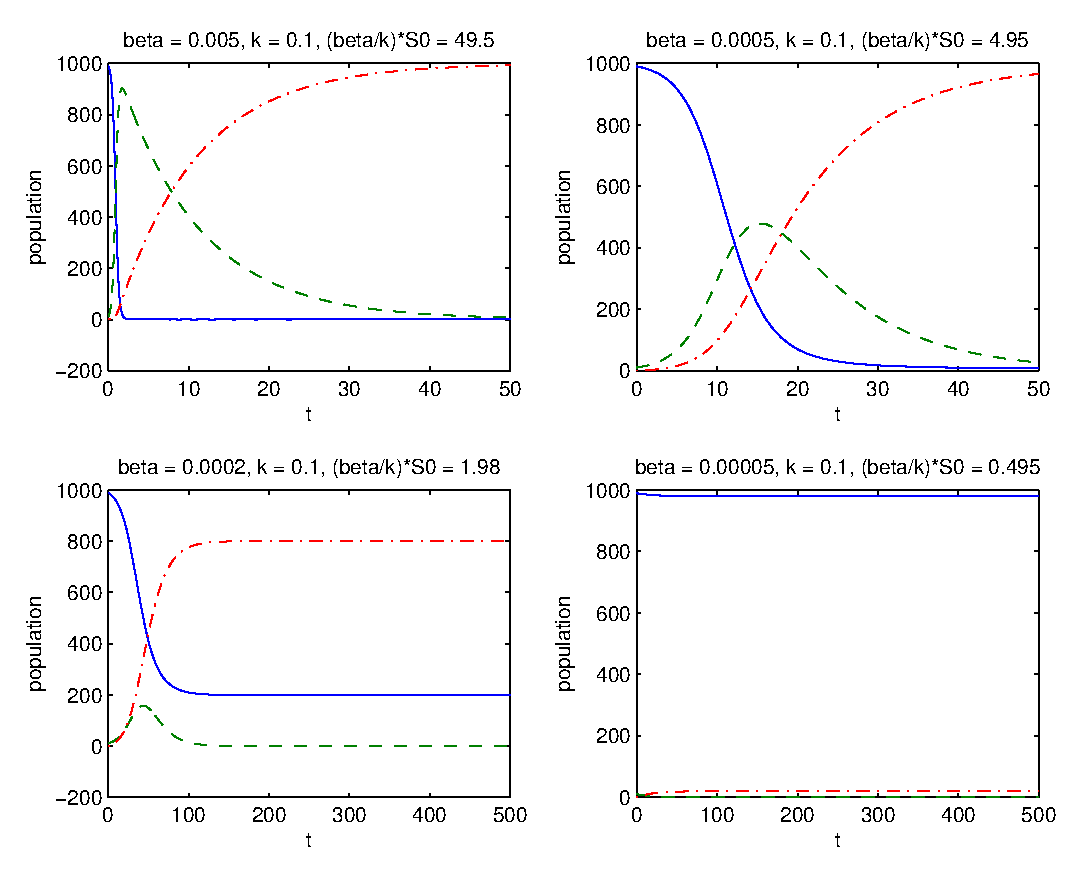
\epsfig{file=sirfig.eps,height=4in}\\
\end{center}
\caption{Number of Susceptibles (solid), Infected (dashed), and Recovered/Dead (dash-dot)
for different basic reproductive ratios $( \beta / k ) S(0)$.}  
\label{fig1}
\end{figure}

From the figure, one can see that if $( \beta / k ) S(0)$ is much greater than $1$,
then the entire population quickly becomes infected and then recovered/dead.
For $( \beta / k ) S(0)$ less than $1$, the infection seems to die out after
only a small percentage of the population has been infected.  For values
somewhat greater than $1$, the number infected and hence later recovered/dead
seems to be a larger fraction but not necessarily all of the population.
The Matlab code used to produce these plots can be found in Appendix A.

\section{Conclusions}
The results of this simple model look fairly reasonable and so they might be
used to decide on a strategy for curtailing an epidemic through vaccinations,
quarantines, etc.  Many enhancements to the model can be made.  For a discussion 
of some of these, see, for example, \cite{Wikipedia}.  

\newpage
\appendix
\section{Matlab Code for Producing Plots}

\begin{verbatim}
global betaglob  % Global variables to be supplied to function sirdot.
global kglob     % Give them funny names so they won't be used elsewhere.

kglob = 0.1;               % Set k.
betas = [.005; .0005; .0002; .0001];
for kase=1:4,
  betaglob = betas(kase);  % Set beta.
  tfinal = 50;  if kase > 2, tfinal = 500; end;
  [tout,sout] = ode45('sirdot',[0 tfinal], [990; 10; 0]); % Solve with ode45.

  subplot(2,2,kase)  
  plot(tout,sout(:,1),'-', tout,sout(:,2),'--', tout,sout(:,3),'-.');
  xlabel('t'), ylabel('population')
  if kase==1,
    title('beta = 0.005, k = 0.1, (beta/k)*S0 = 49.5');
  elseif kase==2,
    title('beta = 0.0005, k = 0.1, (beta/k)*S0 = 4.95');
  elseif kase==3,
    title('beta = 0.0002, k = 0.1, (beta/k)*S0 = 1.98');
  else
    title('beta = 0.00005, k = 0.1, (beta/k)*S0 = 0.495');
  end;
end;

function sirprime = sirdot(t,sir)
global betaglob
global kglob
beta = betaglob;  k = kglob;

sirprime(1,1) = -beta*sir(1)*sir(2);
sirprime(2,1) = beta*sir(1)*sir(2) - k*sir(2);
sirprime(3,1) = k*sir(2);
\end{verbatim}

\newpage

\begin{thebibliography}{99}

\bibitem{Johnson}  Johnson, Teri, {\em Mathematical Modeling of Diseases:
Susceptible-Infected-Recovered (SIR) Model}, Math 4901 Senior Seminar, 
University of Minnesota, Spring 2009.
\verb+http://www.morris.umn.edu/academic/math/Ma4901/Sp09/Final/Teri-Johnson-Final.pdf+ .

\bibitem{Tung} Tung, K.~K., {\em Topics in Mathematical Modeling},
Princeton University Press, 2007.

\bibitem{Wikipedia} Wikipedia, {\em Compartmental models in epidemiology},
\verb+http://en.wikipedia.org/wiki/Compartmental_models_in_epidemiology+ .

\end{thebibliography}
\end{document}


